\documentclass{article}
\usepackage{authblk}
\usepackage[T1]{fontenc}
\usepackage{lmodern}
\usepackage{amsmath}
\usepackage{amssymb}
\usepackage[table,xcdraw]{xcolor}
\usepackage{physics}
\usepackage{siunitx}
\usepackage{float}
\usepackage{wrapfig}
\usepackage{sidecap}
\usepackage{color}
\usepackage{graphicx}
\usepackage{caption}
\usepackage{subcaption}
\usepackage{graphicx}
\usepackage{hyperref}
\usepackage[english]{babel}
\usepackage{multirow}
\usepackage{standalone}
\usepackage[toc,page]{appendix}
\usepackage{listings}
\usepackage{a4wide}
\usepackage{pdfpages}
\usepackage{float}
\usepackage[caption = false]{subfig}
\usepackage{mathtools}
\usepackage[normalem]{ulem}
\usepackage{arydshln}
\useunder{\uline}{\ul}{}
\usepackage[utf8]{inputenc}
\usepackage{relsize}
\usepackage{enumitem}
\usepackage{array}  % in your preamble
\usepackage[most]{tcolorbox}
\usepackage[table]{xcolor}
\numberwithin{equation}{section}
\numberwithin{equation}{subsection}

\title{Notes for Discrete Mathematics (2. Ed) by Rosen: Chapter 1: Logic and Proofs}
\author{Andreas Hansen}
\date{May 2025}

\begin{document}

\maketitle

\section*{\underline{Chapter 1.2: Applications of Propositional Logic} (pg. 17-23)}
\subsection*{Translating English Sentences (pg. 17–18)}
\begin{tcolorbox}[title=Example 1: Translating from English to a Logical Expression]
\textbf{Statement:}  
\begin{center}
\textit{"You can access the Internet from campus only if you are a computer science major or you are not a freshman."}
\end{center}

\textbf{Strategy:}  
Rather than representing the entire sentence as a single propositional variable (e.g. $p$), which would not help in understanding or reasoning, we break it into smaller propositions and connect them using logical operators.

\vspace{1em}

\textbf{Let:}
\begin{itemize}
  \item $a$: You can access the Internet from campus
  \item $c$: You are a computer science major
  \item $f$: You are a freshman
\end{itemize}

\vspace{0.5em}

\textbf{Translation:}
\[
a \rightarrow (c \lor \neg f)
\]
\end{tcolorbox}
\begin{tcolorbox}[title=Example 2: Translating from English to a Logical Expression]
\textbf{Statement:}  
\begin{center}
\textit{"You cannot ride the roller coaster if you are under 4 feet tall unless you are older than 16
years old"}
\end{center}

\textbf{Strategy:}  
Same as previous Example 1. \\ \\
\textbf{Let:}
\begin{itemize}
  \item $q$: You can ride the roller coaster
  \item $r$: You are under 4 feet tall
  \item $s$: You are older than 16 years old
\end{itemize}

\vspace{0.5em}

\textbf{Translation:}
\[
(r \land \neg s) \rightarrow \neg q
\]
\textbf{Explanation:}  \\
The sentence contains an exception with "unless", which in logic means "if not".  \\
So "\textit{unless you are older than 16}" is logically equivalent to "\textit{if you are not older than 16}", or $\neg s$. \\
Thus, the phrase becomes:  
"\textit{If you are under 4 feet tall and not older than 16, then you cannot ride the roller coaster.}"
That is:
\[
(r \land \neg s) \rightarrow \neg q
\]

\end{tcolorbox}



\subsection*{System Specifications (pg. 18-19)}
\begin{tcolorbox}[title=Example 1: Express a specification using logical connectives.]
\textbf{Specification:}  
\begin{center}
\textit{"The automated reply cannot be sent when the file system is full"}
\end{center}
\textbf{Let:}
\begin{itemize}
  \item $p$: The automated reply can be sent
  \item $q$: The file system is full
\end{itemize}
Then we can express the negation of $p$ as $\neg p:$
\begin{center}
\textit{"It is not the case that the automated reply can be sent"} \\ or simply: \textit{"The automated reply cannot be sent"}
\end{center}{}

\vspace{0.5em}

\textbf{Translation (as conditional statement):}
\[
q \rightarrow \neg p
\]
\end{tcolorbox}
\begin{tcolorbox}[colback=white, colframe=gray!60, title=Remark 1]
System specifications should be \textbf{consistent}, that is, they should not contain conflicting requirements
that could be used to derive a contradiction. \\ When specifications are not consistent,
there would be no way to develop a system that satisfies all specifications.
\end{tcolorbox}

\begin{tcolorbox}[title=Example 2: Determine Consistency of System Specifications]
\textbf{Consider the following specifications:}
\begin{enumerate}
    \item \textit{The diagnostic message is stored in the buffer or it is retransmitted.}
    \item \textit{The diagnostic message is not stored in the buffer.}
    \item \textit{If the diagnostic message is stored in the buffer, then it is retransmitted.}
\end{enumerate}

\textbf{Let:}
\begin{itemize}
  \item $p$: The diagnostic message is stored in the buffer
  \item $q$: The diagnostic message is retransmitted
\end{itemize}

\vspace{0.5em}

\textbf{Translations:}
\begin{enumerate}
    \item $p \lor q$
    \item $\neg p$
    \item $p \rightarrow q$
\end{enumerate}

\textbf{Truth Assignment and Evaluation:}

Assume: \( p = \text{F},\ q = \text{T} \)

\begin{itemize}
    \item (1) \( p \lor q = \text{F} \lor \text{T} = \text{T} \)
    \item (2) \( \neg p = \neg \text{F} = \text{T} \)
    \item (3) \( p \rightarrow q = \text{F} \rightarrow \text{T} = \text{T} \) (a conditional with false hypothesis is always true)
\end{itemize}

\textbf{Conclusion:}

Under the assignment \( p = \text{F},\ q = \text{T} \), all three specifications evaluate to true.  \\
\textbf{Therefore, the system specifications are consistent.}

\end{tcolorbox}
\begin{tcolorbox}[title=Example 3: Determine Consistency of System Specifications (2)]
\textbf{Consider the following specifications:}
\begin{enumerate}
    \item \textit{The diagnostic message is stored in the buffer or it is retransmitted.}
    \item \textit{The diagnostic message is not stored in the buffer.}
    \item \textit{If the diagnostic message is stored in the buffer, then it is retransmitted.}
    \item \textit{The diagnostic message is not retransmitted.}
\end{enumerate}

\textbf{Let:}
\begin{itemize}
  \item $p$: The diagnostic message is stored in the buffer
  \item $q$: The diagnostic message is retransmitted
\end{itemize}

\vspace{0.5em}

\textbf{Translations:}
\begin{enumerate}
    \item $p \lor q$
    \item $\neg p$
    \item $p \rightarrow q$
    \item $\neg q$
\end{enumerate}

\textbf{Truth Assignment and Evaluation:}

Assume: \( p = \text{F},\ q = \text{T} \)

\begin{itemize}
    \item (1) \( p \lor q = \text{F} \lor \text{T} = \text{T} \)
    \item (2) \( \neg p = \neg \text{F} = \text{T} \)
    \item (3) \( p \rightarrow q = \text{F} \rightarrow \text{T} = \text{T} \) (a conditional with a false hypothesis is always true)
    \item (4) \( \neg q = \neg \text{T} = \text{F} \) \textbf{← Contradiction!}
\end{itemize}

\textbf{Conclusion:}

Under the truth assignment \( p = \text{F},\ q = \text{T} \), the first three specifications are satisfied.  
However, the fourth specification (\( \neg q \)) is false.  

\textbf{Therefore, the system specifications are inconsistent.}
\end{tcolorbox}



\newpage
\subsection*{Boolean Searches (pg. 19-20)}
\begin{center}
\noindent\fbox{
  \parbox{0.95\linewidth}{
    \textbf{Definition:} \textbf{Boolean searching} refers to a search technique that uses tools called operators and modifiers to limit, widen, and refine your search results
  }
}
\end{center}
\begin{tcolorbox}[colback=white, colframe=gray!60, title=Remark 1]
In Boolean searches, the connective AND is used to match records that contain both of
two search terms, the connective OR is used to match one or both of two search terms, and the
connective NOT (sometimes written as AND NOT ) is used to exclude a particular search term
\end{tcolorbox}
\begin{tcolorbox}[colback=white, colframe=gray!60, title=Remark 2]
\textbf{Web Page Searching}: 
 Most Web search engines support Boolean searching techniques, which
is useful for finding Web pages about particular subjects
\end{tcolorbox}
\begin{tcolorbox}[title=Example 1: Boolean Searching Using Logical Operators]
\textbf{Statement:}  
\begin{center}
\textit{You want to search for Web pages about universities in New Mexico.}
\end{center}

\textbf{Strategy:}  
We can use Boolean logic operators like AND, OR, and NOT to construct search expressions that include only the pages we want. We'll analyze what happens with different Boolean formulations.

\textbf{Let:}
\begin{itemize}
    \item $N$: The page contains the word "NEW"
    \item $M$: The page contains the word "MEXICO"
    \item $U$: The page contains the word "UNIVERSITIES"
\end{itemize}
\textbf{Boolean Search:}
\[
N \land M \land U \ \ \ (\text{Logic operators})
\]
\[
\text{NEW AND MEXICO AND UNIVERSITIES}
\]

This query returns all pages that contain the words "NEW", "MEXICO", and "UNIVERSITIES".
\\
\textbf{Observation:}  
This will include:
\begin{itemize}
    \item Relevant pages about universities in New Mexico (desired)
    \item Irrelevant pages such as ones about "new universities in Mexico" (not desired)
\end{itemize}

\vspace{0.5em}

\textbf{Improved Search Strategy:}  
To reduce irrelevant results, use quotation marks to group the phrase "NEW MEXICO" as a single unit:

\[
\texttt{"NEW MEXICO"} \land U \ \ \text{(Logic operators)}
\]
\[
\text{“NEW
MEXICO” AND UNIVERSITIES.}
\]

This ensures the search engine treats "NEW MEXICO" as a proper phrase and reduces matches like “new universities in Mexico”.

\textbf{Conclusion:}  
Boolean search logic mimics propositional logic. Using grouping (e.g., quotation marks) and appropriate connectives improves search precision.
\end{tcolorbox}

\begin{tcolorbox}[title=Example 2: Boolean Searching with OR and AND Precedence]
\textbf{Statement:}  
\begin{center}
\textit{You want to search for Web pages about universities in either New Mexico or Arizona.}
\end{center}

\textbf{Strategy:}  
We use Boolean logic to capture the intent: pages that mention "universities" and either:
- both "NEW" and "MEXICO", or
- "ARIZONA".
\\ \\
\textbf{Let:}
\begin{itemize}\setlength\itemsep{0em}
    \item $N$: The page contains the word "NEW"
    \item $M$: The page contains the word "MEXICO"
    \item $A$: The page contains the word "ARIZONA"
    \item $U$: The page contains the word "UNIVERSITIES"
\end{itemize}

\textbf{Boolean Search:}
\[
((N \land M) \lor A) \land U
\]
\[
\texttt{(NEW AND MEXICO OR ARIZONA) AND UNIVERSITIES}
\]

\textbf{Note on Precedence:}  
In Boolean logic (and in most search engines), the AND operator has higher precedence than OR.  
So this is interpreted as:
\[
((\text{NEW AND MEXICO}) \text{ OR ARIZONA}) \text{ AND UNIVERSITIES}
\]

\textbf{Observation:}  
This query matches:
\begin{itemize}\setlength\itemsep{0em}
    \item Pages about universities in New Mexico (contain NEW, MEXICO, and UNIVERSITIES)
    \item Pages about universities in Arizona (contain ARIZONA and UNIVERSITIES)
    \item But also possibly irrelevant pages such as:
    \begin{itemize}\setlength\itemsep{0em}
        \item Pages with NEW and MEXICO but not universities
        \item Pages about Arizona universities not specifically comparing them with New Mexico
    \end{itemize}
\end{itemize}

\vspace{0.5em}

\textbf{Improved Search Strategy:}  
Use grouping with parentheses or quotation marks to better control matching, especially when using search engines like Google:

\[
\texttt{"NEW MEXICO" OR ARIZONA AND UNIVERSITIES}
\]

This still depends on how the search engine parses precedence. Some engines may interpret it as:
\[
\texttt{"NEW MEXICO"} \lor (\texttt{ARIZONA} \land \texttt{UNIVERSITIES})
\]
which may not be what you want.
\\ \\
\textbf{Conclusion:}  
Operator precedence matters in Boolean search. To refine results, group expressions using parentheses or quotes, and be aware that not all engines use the same precedence rules.
\end{tcolorbox}

\begin{tcolorbox}[title=Example 3: Boolean Searching Using NOT (Exclusion)]
\textbf{Statement:}  
\begin{center}
\textit{You want to find Web pages about universities in Mexico, but exclude those about New Mexico.}
\end{center}

\textbf{Strategy:}  
A naive search for \texttt{MEXICO AND UNIVERSITIES} will match both:
\begin{itemize}\setlength\itemsep{0em}
    \item Pages about universities in Mexico (desired)
    \item Pages about universities in New Mexico (undesired)
\end{itemize}

To avoid including pages that mention “NEW”, we use the \textbf{NOT} operator to exclude them.

\vspace{0.5em}

\textbf{Let:}
\begin{itemize}\setlength\itemsep{0em}
    \item $M$: The page contains the word "MEXICO"
    \item $U$: The page contains the word "UNIVERSITIES"
    \item $N$: The page contains the word "NEW"
\end{itemize}

\textbf{Boolean Search:}
\[
(M \land U) \land \neg N
\]
\[
\texttt{(MEXICO AND UNIVERSITIES) NOT NEW}
\]

\textbf{Observation:}  
This search will include:
\begin{itemize}\setlength\itemsep{0em}
    \item Pages that mention both “MEXICO” and “UNIVERSITIES”
    \item But \textbf{exclude} any pages that also contain the word “NEW” — removing false positives related to "New Mexico"
\end{itemize}

\vspace{0.5em}

\textbf{Search Engine Note:}  
Many engines like Google do not use the word \texttt{NOT}, but instead use the minus sign (\texttt{-}) to indicate exclusion.
\\ \\
\textbf{Google-style equivalent:}
\[
\texttt{MEXICO UNIVERSITIES -NEW}
\]

\textbf{Conclusion:}  
The NOT operator (or \texttt{-} in practice) is useful in Boolean searching for filtering out results that include unwanted keywords. When searching for content that overlaps with similar terms, this exclusion strategy improves result relevance.
\end{tcolorbox}


\newpage
\subsection*{Logic Puzzles (pg. 20-22)}
\begin{tcolorbox}[title=Example 1: King's Daughter Treasure Logic Puzzle (1/2)]
\textbf{Puzzle:}  
\begin{itemize}
    \item As a reward for saving his daughter from pirates, the King has given you the opportunity to win
a treasure hidden inside one of three trunks. 
    \item The two trunks that do not hold the treasure are
empty. 
    \item To win, you must select the correct trunk. \item Trunks 1 and 2 are each inscribed with the
message “\textit{This trunk is empty,}” and Trunk 3 is inscribed with the message “\textit{The treasure is in
Trunk 2.}” 
    \item The Queen, who never lies, tells you that only one of these inscriptions is true, while
the other two are wrong. 
    \item Which trunk should you select to win?
\end{itemize}{}

\textbf{Strategy:}  
Let $p_i$ be the proposition that the treasure is in Trunk $i$, for $i = 1, 2, 3$. To translate into
propositional logic the Queen’s statement that exactly one of the inscriptions is true, we observe
that the inscriptions on Trunk 1, Trunk 2, and Trunk 3, are:
\begin{center}
$\neg p_1 \ \ \  \text{(Not in Trunk 1)} $ \\
$\neg p_2 \ \ \  \text{(Not in Trunk 2)} $ \\
$p_2 \ \ \  \text{(In Trunk 2)} $ \\
\end{center}
Then we have to construct the 3 different scenarios:
\begin{itemize}
    \item Inscription in Trunk 1 is correct:
    \begin{center}
$\neg p_1 \land \neg(\neg p_2) \land \neg p_2$    
\end{center}
   \item Inscription in Trunk 2 is correct:
    \begin{center}
$\neg (\neg p_1) \land \neg p_2 \land \neg p_2$    
\end{center}
    \item Inscription in Trunk 3 is correct:
    \begin{center}
$\neg (\neg p_1) \land \neg (\neg p_2) \land p_2$    
\end{center}
\end{itemize}
Only one scenario can be correct, so we have to combine them with the disjunction operator $\lor$ and we get:
\begin{center}
$\left( \neg p_1 \land \neg(\neg p_2) \land \neg p_2 \right) \lor \left(\neg (\neg p_1) \land \neg p_2 \land \neg p_2 \right) \lor \left(\neg (\neg p_1) \land \neg (\neg p_2) \land p_2 \right) $    
\end{center}
\textbf{Reducing and simplifying (1/2):}
\begin{center}
$\neg (\neg p_i) = p_i $    
\end{center}
\begin{center}
$\left( \neg p_1 \land p_2 \land \neg p_2 \right) \lor \left(p_1 \land \neg p_2 \land \neg p_2 \right) \lor \left(p_1 \land  p_2 \land p_2 \right) $    
\end{center}
\begin{center}
$\left(p_1 \land \neg p_2  \right) \lor \left(p_1 \land  p_2\right) $    
\end{center}
Now using distributive law: $p_1 \land (\neg p_2 \lor p_2) $ 
\end{tcolorbox}
\begin{tcolorbox}[title=Example 1: King's Daughter Treasure Logic Puzzle (2/2)]
\textbf{Reducing and simplying (2/2):}  
\begin{center}
$\left(p_1 \land \neg p_2  \right) \lor \left(p_1 \land  p_2\right) = p_1 \land (\neg p_2 \lor p_2) $    
\end{center}
But we know that it has to be true that either $\neg p_2$ or $p_2$ and we can denote this as
\begin{center}
$\neg p_2 \lor p_2 = \mathbf{T}$   
\end{center}
This gives
\begin{center}
$p_1 \land (\neg p_2 \lor p_2) = p_1 \land \mathbf{T}$ 
\end{center}
But this is equivalent to
\begin{center}
$ p_1 \land \mathbf{T} = p_1$ 
\end{center}
\textbf{Conclusion:} \\
So the treasure is in Trunk 1 (that is, $p_1$ is true), and $p_2$ and $p_3$ are false; and the inscription on Trunk 2 is the only true one.
\end{tcolorbox}

\begin{tcolorbox}[title=Example 2: Raymond Smullyan´s Knights and Knaves]
\textbf{Puzzle:}  
\begin{itemize}
    \item In [Sm78] Smullyan posed many puzzles about an island that has two kinds of inhabitants,
knights, who always tell the truth, and their opposites, knaves, who always lie.
    \item You encounter two people A and B.
    \item What are A and B if A says “\textit{B is a knight}” and B says “T\textit{he two of us are
opposite types”?} 
\end{itemize}{}

\textbf{Strategy:}  
Let $p$ and $q$ be the statements that A is a knight and B is a knight, respectively, so that
\begin{center}
$\neg p \ \ \ \text{(A is a knave)} $ \\
$\neg q \ \ \ \text{(B is a knave)}$
\end{center}
Then we have to construct the 2 different scenarios:
\begin{itemize}
    \item \textbf{A is a knight and tells the truth:}\\
    Then $p$ is True, and B is also a knight ($q$ is True) and tells the truth. \\ But that means the statement $B$ says also has to be true and this cannot be, since they are the same type. So this scenario is impossible and both A and B can´t be knights
    \item \textbf{A is a knave and lies:} \\
    Then A lies about B being a knight. This means that B also must be a knave. This also works when looking at B´s statement, because B also lies that the are different types. 
\end{itemize}
\textbf{Conclusion:} \\
We can conclude that both A and B are
knaves.
 
\end{tcolorbox}

\begin{tcolorbox}[title=Example 3: Muddy children puzzle]
\textbf{Puzzle:}  
\begin{itemize}
    \item A father tells his two children, a boy and a girl, to play in their backyard without getting dirty. However, while playing, both children get mud on their foreheads
    \item When the children stop playing,
the father says “A\textit{t least one of you has a muddy forehead,}” and then asks the children to
answer “\textit{Yes}” or “\textit{No}” to the question: \textit{“Do you know whether you have a muddy forehead?}”
    \item The father asks this question twice. 
    \item What will the children answer each time this question is asked, assuming that a child can see whether his or her sibling has a muddy forehead, but cannot see his or her own forehead?
    \item Assume that both children are honest and that the children answer each question simultaneously.
\end{itemize}

\textbf{Strategy:}  
Let $s$ be the statement that the son has a muddy forehead and let $d$ be the statement that
the daughter has a muddy forehead. 
\\ \\ 
When the father says that at least one of the two children
has a muddy forehead, he is stating that the disjunction is true
\begin{center}
$s \lor d$
\end{center}
Then we have to construct the 2 different times the father asks:
\begin{itemize}
    \item \textbf{Round 1:}\\
    We assum that each children tells the true and at the same time, so they would both answer "\textit{No}", since the son only knows $d$ is true and daughter only knows $s$ is true. 
    \item \textbf{Round 2:}\\
    Each child now knows that they themselves must have mud on their forehead, since they both answered "\textit{No}" on the 1. question and the father stated that at least one of them has a muddy forehead. \\ \\ They are both going to answer "\textit{Yes}" this time.
\end{itemize}
\textbf{Conclusion:} \\
First time the father asks, both children answer "\textit{No}". \\ Second time the father asks, both children answer "\textit{Yes}".
 
\end{tcolorbox}



\newpage
\subsection*{Logic Circuits (pg. 22-23)}
\begin{tcolorbox}[title=Definition: Logic circuit (digital circuit)]
Receives input signals $p_1, p_2,\ldots, p_n$, each a bit [either 0 (off) or 1 (on)], and produces output signals $s_1, s_2,\ldots, s_n$, each a bit.  
\end{tcolorbox}
\begin{tcolorbox}[colback=white, colframe=gray!60, title=Remark 1]
In this section we will
restrict our attention to logic circuits with a single output signal; in general, digital circuits may
have multiple outputs.
\end{tcolorbox}
\begin{tcolorbox}[title=Definition: Basic Logic Gates]
Complicated digital circuits can be constructed from three basic circuits, called gates:

\begin{enumerate}
    \item The \textbf{inverter}, or \textbf{NOT gate}, takes an input bit $p$ and produces as output $\neg p$.
\begin{center}
    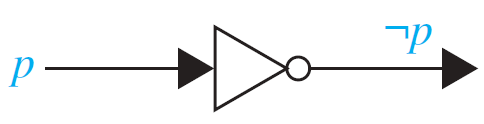
\includegraphics[width=0.3\linewidth]{chp1_2_applogic/inv.png}
\end{center}
    \item The \textbf{OR gate} takes two input signals $p$ and $q$, each a bit, and produces as output the signal $p\lor q$.
\begin{center}
    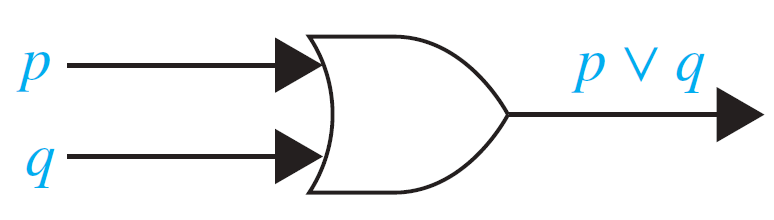
\includegraphics[width=0.3\linewidth]{chp1_2_applogic/or.png}
\end{center}
    \item The \textbf{AND gate} takes two input signals $p$ and $q$, each a bit, and produces as output the signal $p\land q$.
\begin{center}
    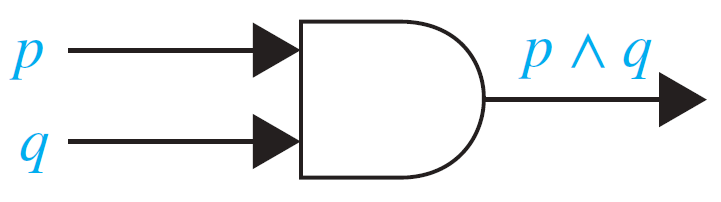
\includegraphics[width=0.3\linewidth]{chp1_2_applogic/and.png}
\end{center}
\end{enumerate}
\end{tcolorbox}

\begin{tcolorbox}[title=Example 1: Output for the combinatorial circuit]
Determine the output for the combinatorial circuit
\begin{center}
    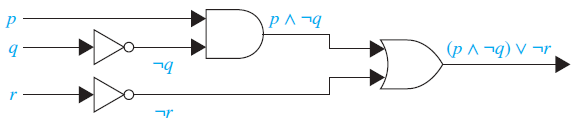
\includegraphics[width=0.6\linewidth]{chp1_2_applogic/comb1.png}
\end{center}
\textbf{Strategy:}
We display the output of each logic gate in the circuit
\begin{itemize}
    \item We see that the \textbf{AND gate} takes input of $p$ and $\neg q$, the output of the inverter with input $q$, and produces $p \land \neg q$
    \item Next, we note that the \textbf{OR gate} takes input $p \land \neg q$ and $\neg r$ (the output of the inverter with
input $r$), and produces the final output $(p \land \neg q) \lor \neg r$ .
\end{itemize}
\end{tcolorbox}
\begin{tcolorbox}[title=Example 2: Combinatorial circuit when want a certain output]
Build a digital circuit that produces the output 
\begin{center}
$\left(p \lor \neg r \right) \land \left(\neg p \lor (q \lor \neg r) \right)$    
\end{center}
when given input bits $p$, $q$, and $r$. \\ \\
\textbf{Strategy:}
We start with the output and "work backwards"
\begin{itemize}
    \item \textbf{Output}: $\left(p \lor \neg r \right) \land \left(\neg p \lor (q \lor \neg r) \right)$ is a conjunction (\textbf{AND gate}) between $\left(p \lor \neg r \right)$ and $\left(\neg p \lor (q \lor \neg r) \right)$
    \item $\mathbf{p \lor \neg r }$ : This is a disjunction (\textbf{OR gate}) between $p$ and $\neg r$
    \item $\mathbf{\neg r}$: This is a negation (\textbf{Inverter/NOT gate}) of $r$
    \item $\mathbf{\neg p \lor (q \lor \neg r) }:$ This is a disjunction (\textbf{OR gate}) between $\neg p$ and $q \lor \neg r$
    \item $\mathbf{\neg p}$: This is a negation (\textbf{Inverter/NOT gate}) of $p$
    \item $\mathbf{q \lor \neg r}:$ This is a disjunction between $q$ and $\neg r$
\end{itemize}
\textbf{Conclusion and figure:}
\begin{center}
    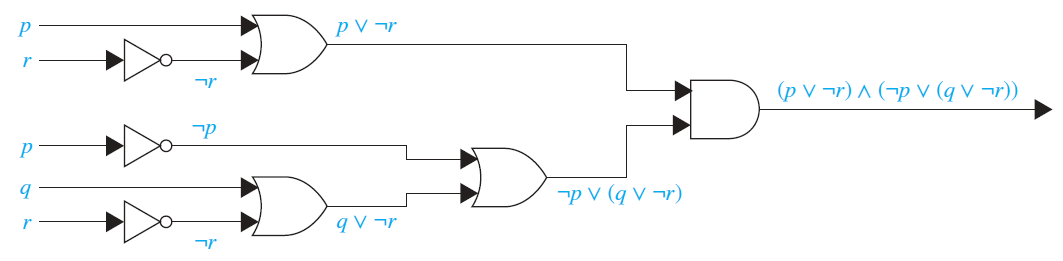
\includegraphics[width=0.9\linewidth]{chp1_2_applogic/comb2.png}
\end{center}
\end{tcolorbox}
















\end{document}
